\documentclass[
	ngerman,
	ruledheaders=section,
	class=report,
	thesis={type=Seminararbeit}, %Möglichkeiten: Seminararbeit, bachelor, master
	accentcolor=2d,
	marginpar=false,
	BCOR=5mm,
	parskip=half-,
	fontsize=12pt
]{tudapub}

% Achtung: Diese Vorlage verwendet biblatex. Bitte wählt biber in eurem Editor als Literaturverzeichnis-Compiler aus.

\addTitleBoxLogo*{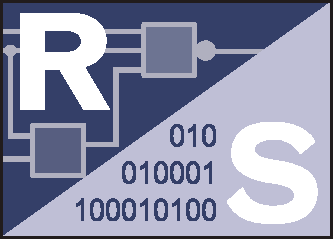
\includegraphics[width=\linewidth,trim=-1.05cm -0.5cm -4.45cm -0.5cm]{bilder/rs_logo}}

% Der folgende Block ist nur bei pdfTeX auf Versionen vor April 2018 notwendig
\usepackage{iftex}
\ifPDFTeX
\usepackage[utf8]{inputenc}
\fi

%%%%%%%%%%%%%%%%%%%
%Sprachanpassung & Verbesserte Trennregeln
%%%%%%%%%%%%%%%%%%%
\usepackage[english, main=ngerman]{babel}
\usepackage[autostyle]{csquotes}% Anführungszeichen vereinfacht
\usepackage{microtype}

%%%%%%%%%%%%%%%%%%%
%Literaturverzeichnis
%%%%%%%%%%%%%%%%%%%
\usepackage{biblatex}
\bibliography{Literaturverzeichnis}

%%%%%%%%%%%%%%%%%%%
%Tabellen
%%%%%%%%%%%%%%%%%%%
%\usepackage{array}     % Basispaket für Tabellenkonfiguration, wird von den folgenden automatisch geladen
\usepackage{tabularx}   % Tabellen, die sich automatisch der Breite anpassen
%\usepackage{longtable} % Mehrseitige Tabellen
%\usepackage{xltabular} % Mehrseitige Tabellen mit anpassarer Breite
\usepackage{booktabs}   % Verbesserte Möglichkeiten für Tabellenlayout über horizontale Linien

%%%%%%%%%%%%%%%%%%%
%Paketvorschläge Mathematik
%%%%%%%%%%%%%%%%%%%
%\usepackage{mathtools} % erweiterte Fassung von amsmath
%\usepackage{amssymb}   % erweiterter Zeichensatz
%\usepackage{siunitx}   % Einheiten

%%%%%%%%%%%%%%%%%%%
%RS Vorlage
%%%%%%%%%%%%%%%%%%%
\usepackage{acronym}
\usepackage{listings}

\lstset{language=C,basicstyle=\small, breaklines=true, showtabs=false, showspaces=false, showstringspaces=false}

\renewcommand{\lstlistingname}{Quelltext}
\lstset{literate=%
	{Ö}{{\"O}}1
	{Ä}{{\"A}}1
	{Ü}{{\"U}}1
	{ß}{{\ss}}1
	{ü}{{\"u}}1
	{ä}{{\"a}}1
	{ö}{{\"o}}1
}

\begin{document}

\Metadata{
	title=Titel der Thesis,
	author=Student*in
}

\title{Titel der Thesis}
\subtitle{Untertitel} %optional
\author[M. Mustermann]{Student*in} %optionales Argument ist die Signatur, bitte auch anpassen

\department{etit}
\institute{Institut für Datentechnik}
\group{FG Rechnersysteme}

\reviewer{Prof. Dr.-Ing. Christian Hochberger \and M.Sc. Betreuer*in}

\submissiondate{\today}
\examdate{\today}

%	\tuprints{urn=1234,printid=12345}
%	\dedication{Für alle, die \TeX{} nutzen.}

\maketitle

\affidavit % Bei Seminararbeiten ist die Eigenständigkeitserklärung nicht notwendig und kann auskommentiert werden.

\tableofcontents

\chapter{Einleitung}

\textit{kursiver Text} \\
\texttt{besonderer Text} \\
normaler Text
\begin{itemize}
\item[\textbf{1)}] \textbf{Aufzählung1}\\
Text der Aufzählung
\item [\textbf{2)}]\textbf{Aufzählung2}
\item [\textbf{3)}]\textbf{Aufzählung3}
\item [\textbf{4)}]\textbf{Aufzählung4}
\item [\textbf{5)}]\textbf{Aufzählung5}
\end{itemize}
Quellenverlinkung \cite{UCS_XDL_UseCaseSenarios}


\chapter{Verwendete Formate \& Programme}

\section{Executable and Linking Format}

\section{SpartanMC Hex Format}

\section{make-toolchain}

\begin{figure}[h] 
\centering
\includegraphics[width=0.5\linewidth]{example-image-a}
\caption{Dies ist eine Caption}
\label{fig:example_image}
\end{figure}
\chapter{Implementierung}

\begin{lstlisting}
inst "subsystem_0/spartanmc_0/ifid/memory/MEM_BL[0].DPRAMA"
 INITP_00::d8aa100063c47860a000003c49c07832c10491802825301224b24c5014400024
 INITP_01::0000030048018d68a923f02b84b0d9462112c00611594c22a96186c986d31e03
  INIT_00::000035a500a4011000a000000000000000000000000000002015221600051f00
  INIT_01::8015648415fe0880ff1564884600863f0084370080822200016401ff1f9e012c
  INIT_02::1525500040009d001514ff8000fe156401156485a0821507018015648215fe01
  INIT_03::dfff800001001505c50215251525a505ff811564020015f6ff8000010015e50e
  INIT_04::01a580156401156490b00390850615ac0985ffd0811015ac0985ffd08085e915
  INIT_05::6480bc016715736415787015752d15ec6f7e156f30011815ec09ffd085ffc080
  INIT_06::62ceeb15ec09ffd085ffc08001da15ec09ffd085ffc080012085bdc534153015
  INIT_07::85ffc08587c58002a5156480b601cb1525154bd015ac583415582d15ec625115
  INIT_08::855504a515648542e5c5a5a815649bc330ec09ffd085ffc080013915ec09ffd0
  INIT_09::6d308280bc0180ff1564853f01a51564854503a51564856fe5c5a51564a51564
  INIT_0A::8506c5ff00a5156415c58582842200ff15640015fbff800115a55000150bff80
  INIT_0B::00139300000e00ffa401e5ffc51564a5f385ac1a008c2d0e0031019f15648537
  INIT_0C::2030001b00ce01c5ff1564853521001564853bf58000a6e0f0be01d485ffff21
  INIT_0D::41004030e315d8d80102ff0115044005f8ff8a9085f08501013092019f10408a
  INIT_0E::31b8003fb400000a216c6f206c651564fb150080ffff04ff15648504ffa51b00
INIT_0F::00000000000000000000000000000000000000010a64e810a046444239373533 ;
\end{lstlisting}

\chapter{Benutzungshinweise}
\chapter{Evaluation}
\begin{itemize}
\item \textbf{Änderungsmöglichkeiten kleinerer Art}
\begin{itemize}
\item[-] Löschen einer Funktion
\item[-] Hinzufügen einer Funktion
\item[-] Umbenennen einer Funktion
\item[-] Ändern des Körpers einer Funktion 
\end{itemize}
\end{itemize}
Diese Änderungen kleinerer Art führten bei meiner Programmierung zu korrekten Ergebnissen.
\begin{itemize}
\item \textbf{Funktionalitätsänderungen}
\begin{itemize}
\item[-] Ein kleines Programm in ein großes Programm ändern.
\item[-] Ein großes Programm zu einem anderen großen Programm ändern.
\item[-] Ein großes Programm in ein kleines Programm ändern.
\end{itemize}
\end{itemize}

\chapter{Zusammenfassung}


\section*{Abkürzungsverzeichnis}
\begin{acronym}
	\acro{CLB}{Configurable Logic Block}
	\acro{CPU}{central processing unit}
	\acro{ELF}{Executable and Linking Format}
	\acro{FPGA}{Field Programmable Gate Array}
	\acro{MC}{Microcontroller}
	\acro{CPU}{central processing unit}
	\acro{NCD}{Native Circuit Description Format}
	\acro{SoC}{System on Chip}
	\acro{Sph}{SpartanMC Hex Dateiformat}
	\acro{XDL}{Xilinx Design Language Format}
\end{acronym}

\listoffigures	

\nocite{*}
\printbibliography
	
\end{document}
